\documentclass[aps,onecolumn,11pt]{revtex4}
\usepackage{graphicx}
\usepackage{amssymb,amsfonts,amsmath,amsthm}
\usepackage{chemarr}
\usepackage{bm}
\usepackage{pslatex}
\usepackage{xfrac}
\usepackage[dvipsnames]{xcolor}
%\usepackage{bookman}
\usepackage{dsfont}
\usepackage{mathptmx}
\usepackage{hyperref}
%\usepackage{rotating}

%%%%%%%%%%%%%%%%%%%%%%%%%%%%%%%%%%%%%%%%%%%%%%%%%%%%%%%%%%%%%%%%%%%%%%%%%%%%%%
%%
%%
%% Style
%%
%%
%%%%%%%%%%%%%%%%%%%%%%%%%%%%%%%%%%%%%%%%%%%%%%%%%%%%%%%%%%%%%%%%%%%%%%%%%%%%%%
\newcommand{\mychem}[1]{\mathtt{#1}}
\newcommand{\myconc}[1]{\left\lbrack{#1}\right\rbrack}

\newcommand{\spLi}[1]{{~^{\mychem{#1}}\mychem{Li}}}
\newcommand{\Li}[1]{\myconc{\spLi{#1}}}

\newcommand{\spEout}{\mychem{E}}
\newcommand{\Eout}{\myconc{\spEout}}

%\newcommand{\spLiEin}[1]{\left\lbrace\spLi{#1}\spEout\right\rbrace_{\mathrm{in}}}
%\newcommand{\LiEin}[1]{\myconc{\spLiEin{#1}}}

\newcommand{\spLiE}[1]{\left\lbrace\spLi{#1}\spEout\right\rbrace}
\newcommand{\LiE}[1]{\myconc{\spLiE{#1}}}


%\newcommand{\spLiEout}[1]{\left\lbrace\spLi{#1}\spEout\right\rbrace_{\mathrm{out}}}
%\newcommand{\LiEout}[1]{\myconc{\spLiEout{#1}}}

\newcommand{\spLiIn}[1]{{\spLi{#1}}_{\mathrm{in}}}
\newcommand{\LiIn}[1]{\myconc{\spLiIn{#1}}}

\newcommand{\spLiOut}[1]{{\spLi{#1}}_{\mathrm{out}}}
\newcommand{\LiOut}[1]{\myconc{\spLiOut{#1}}}

\newcommand{\spEHin}{\mychem{EH}}
\newcommand{\EHin}{\myconc{\spEHin}}
\newcommand{\spproton}{\mychem{H}}
\newcommand{\proton}{\myconc{\spproton}}

\newcommand{\mytrn}[1]{{#1}^{\!\mathsf{T}}}
\newcommand{\mymat}[1]{{\bm{#1}}}
\newcommand{\mydet}[1]{{\left|{#1}\right|}}

\newcommand{\ratioLi}{ {\left(\dfrac{\Li{7}}{\Li{6}}\right)} }
\newcommand{\deltaLi}{ {\delta\!\!\!\spLi{7}} }
\newcommand{\deltaLiOut}{{\deltaLi}_{\mathrm{out}}}

\newcommand{\LiAll}{\Lambda}
\newcommand{\LiAllOut}{{\LiAll}_{\mathrm{out}}}

\newcommand{\NHE}[1]{\mychem{NHE}{\mychem{\hbox{-}\!#1}}}
\newcommand{\todo}[1]{\framebox{\textbf{\color{WildStrawberry}{#1}}}}
\newcommand{\ko}{\dagger}


%%%%%%%%%%%%%%%%%%%%%%%%%%%%%%%%%%%%%%%%%%%%%%%%%%%%%%%%%%%%%%%%%%%%%%%%%%%%%%
%%
%%
%% Document
%%
%%
%%%%%%%%%%%%%%%%%%%%%%%%%%%%%%%%%%%%%%%%%%%%%%%%%%%%%%%%%%%%%%%%%%%%%%%%%%%%%%


\begin{document}
\title{Supplementary Material...}
\maketitle

\section{Setting up the Model}

\subsection{Description And Notations}

\subsubsection{Isotopic Ratio}
The isotopic separation of a mixture of $\spLi{6}$ and $\spLi{7}$ is defined by:
\begin{equation}
	\deltaLi = \left(
		\dfrac{\left(\dfrac{\Li{7}}{\Li{6}}\right)_{sample}}
		{\left(\dfrac{\Li{7}}{\Li{6}}\right)_{standard}}
		 -1 
	\right) \times 1000,
\end{equation}
or
\begin{equation}
	\left(\dfrac{\Li{7}}{\Li{6}}\right)_{sample} = \left(\dfrac{\Li{7}}{\Li{6}}\right)_{standard} \left[1+10^{-3}\deltaLi\right] = \lambda_s \left[1+10^{-3}\deltaLi\right].
\end{equation}
We define
\begin{equation}
\left\lbrace
\begin{array}{rclcl}
	\LiAll & = & \Li{6} + \Li{7}\\
	\Li{6} & = & \dfrac{1}{1+\lambda_s \left[1+10^{-3}\deltaLiOut\right] } \LiAllOut & = & \epsilon_6 \LiAllOut   \\
	\\
	\Li{7} & = & \dfrac{\lambda_s \left[1+10^{-3}\deltaLiOut\right]}{1+\lambda_s \left[1+10^{-3}\deltaLiOut\right] } \LiAllOut & = & \epsilon_7 \LiAllOut\\
\end{array}
\right.
\end{equation}

For the presented experiments, the lithium composition is:
\begin{equation}
	\lambda_s = 12.0192, \; \deltaLi = 14.57 \Rightarrow \epsilon_6 \simeq 0.076,\;\epsilon_7 \simeq 0.924
\end{equation}


\subsubsection{Lithium Transport}

Let us describe how a cell may intake a lithium isotope from the outer medium, which is formally described by the transformation
of $\spLiOut{x}$ into $\spLi{x}$ for $x=\lbrace 6,7 \rbrace$. We distinguish two main paths.

\begin{itemize}
\item We assume that the Enzymatic Path, using $\NHE{1}$ as the enzyme $\spEout$ works as follows. A more detailed description is found in \todo{ref}.
	\begin{itemize}
	\item The outer lithium is associated with a membrane enzyme:
	\begin{equation}
		\label{eq:pre}
		\spLiOut{x} + \spEout  \xrightleftharpoons[~~k^d_x~~]{~~k^a_x~~} \spLiE{x},
	\end{equation}
	where $k^a_x$ and $k^d_x$ respectively are the association and the dissociation rate constants.
	
	\item Then the associated complex exchange an inner proton with a lithium ion:
	\begin{equation}
		\label{eq:xch}
		\spLiE{x} + \spproton   \xrightleftharpoons[~~k^q_x~~]{~~k^p_x~~}   \spEHin + \spLi{x}, 
	\end{equation}
	where $k^p_x$ and $k^q_x$ respectively are the forward and reverse protonation rate constants.
	
	\item The attached inner proton is then transported out of the cell to recycle the enzyme:
	\begin{equation}
			\spEHin   \xrightarrow{~~k_h~~}   \spEout + \spproton_{\mathrm{out}} 
	\end{equation}	
	where $k_h$ is the  apparent recycling constant rate, assuming that $\spEHin$ is the predominant form of the enzyme at the inner membrane surface \todo{Lacroix EMBO 2004 fig 3A}.
	\end{itemize}

\item The Passive Path (or Leak) consists in the use by the lithium species of some ion channels, following the electro-osmotic gradient as described by the Goldman-Hodkins-Katz \todo{ref} equations and leading to:
	\begin{equation}
	\label{eq:ghk}
		\spLiOut{x} \xrightleftharpoons[~~k_x~~]{~~k_x e^{-\frac{FV_m}{RT}}~~}   \spLi{x} 
	\end{equation}
where $V_m$ is the membrane potential, $F$ is the Faraday's constant, $R$ is the perfect gas constant, and $T$ is the absolute temperature.

\end{itemize}

\subsubsection{Internal Proton Concentration}
Even if we account here the proton as a transported species, it is also a reactive species which is involved in many reactions, as to ensure the cell homeostasis\todo{ref}. That is why we consider $\proton$ as a heuristic function of time, which will very depend on the full cell pH regulation process.

\subsubsection{Membrane Potential Regulation}
The full system is electroneutral, since it globally exchanges one $\spproton$ per one $\spLi{x}$. Though the Nernst's potential and currents are likely to be displaced \todo{more explanations?}

\subsection{Full Kinetic Scheme}
We define the 11 following rates:
\begin{equation}
	\label{eq:rates}
\left\lbrace
\begin{array}{rcl}
	v^a_x & = & k^a_x \Eout \LiOut{x} \\
	\\
	v^d_x & = & k^d_x \LiE{x} \\
	\\
	v^p_x & = & k^p_x \LiE{x} \proton\\
	\\
	v^q_x & = & k^q_x \Li{x} \EHin\\
	\\
	v_h   & = & k_x \EHin\\
	\\
	v^l_x & = & k_x\left(\Theta \LiOut{x} - \Li{x}\right),\;\;\Theta = e^{-\frac{FV_m}{RT}}\\
\end{array}
\right.
\end{equation}
We deduce the full constrained kinetic scheme with 6 variables:
\begin{equation}
	\label{eq:full}
\left\lbrace
\begin{array}{rcl}
\partial_t \EHin & = & -v_h + \sum_x\left(v^p_x - v^q_x\right)\\
\\
\partial_t \Eout & = & v_h + \sum_x(v^a_x -v^d_x)\\
\\
\partial_t \LiE{x} & = & v^a_x -v^d_x + v^q_x -v^p_x\\
\\
\partial_t \Li{x}  & = & v^l_x + v^p_x - v^q_x\\
\end{array}
\right.
\end{equation}
and we check that we always verify the conservation:
\begin{equation}
	E_0  =  \Eout + \EHin + \LiE{6} + \LiE{7},
\end{equation}
where $E_0$ is the cellular total $\NHE{1}$ membrane concentration.

\subsection{Complexity Reduction by Semi-Stationary Kinetic Scheme}

\subsubsection{Algebraic Simplification}
We assume that the binding of the outer lithium to the enzyme is fast compared to its subsequent transport through the membrane. 
Accordingly, we define the two equilibria:
\begin{equation}
\label{eq:J}
\spLiOut{x} +  \spEout    \xrightleftharpoons[]{}  \spLiE{x}, \;\; J_x = \dfrac{\LiE{x}}{\LiOut{x} \Eout} = \dfrac{k_x^a}{k_x^d},
\end{equation}
which shall be always verified.
We now harness the algebraic method previously established\todo{ref} to end up with only 3 coupled equations:
\begin{equation}
\label{eq:sys}
\left\lbrace
	\begin{array}{rcl}
		\partial_t\EHin & = & -k_h \EHin + \left(E_0- \EHin\right) \dfrac{\proton}{\mathfrak{D}} \left(\sum_x k_x^p J_x\LiOut{x} \right)  
		- \EHin \left({\sum_x k_x^q \Li{x}} \right)
		\\
		\\
		& = & 
		-k_h E_0+ \left(E_0- \EHin\right)\left\lbrack k_h+ \dfrac{\proton}{\mathfrak{D}} \left(\sum_x k_x^p J_x\LiOut{x}\right)\right] 
		- \EHin \left( {\sum_x k_x^q \Li{x}} \right)
		\\
		\\
		\partial_t\Li{x} & = & k_x \left(\Theta\LiOut{x} -\Li{x} \right)  + \left(E_0-\EHin\right) \dfrac{\proton}{\mathfrak{D}}   k_x^p  J_x \LiOut{x}  
		- \EHin k_x^q \Li{x}
		\\
		\\
		(\mathfrak{D} & = & 1+\sum_x J_x \LiOut{x} )\\
	\end{array}
\right.
\end{equation}

\subsubsection{Rescaling and rewriting}
We define the following set of variables:
\begin{equation}
\label{eq:scale}
\left\lbrace
\begin{array}{rcll}
	\alpha & = & \dfrac{\EHin}{E_0} & \text{(fraction of protonated enzyme)}\\
	\\
	\hat\alpha & = & 1-\alpha       & \text{(fraction of not protonated enzyme)}\\
	\\
	\beta_x    & = & \dfrac{\Li{x}}{\LiOut{x}} & \text{(internal lithium amplification factor)}\\
	\\
	J_\epsilon & = & \sum_x \epsilon_x J_x & \text{(mixed affinity)}\\
	\\
	\LiAllOut  & = & \LiOut{6} + \LiOut{7} & \text{(external lithium concentration)}\\
\end{array}
\right..
\end{equation}
Then we rewrite:
\begin{equation}
\label{eq:sysnew}
\left\lbrace
\begin{array}{rcl}
	\partial_t \alpha & = & -k_h \alpha + \LiAllOut \left[ (1-\alpha) \proton  \dfrac{ \left(\sum_x k^p_x \epsilon_x J_x\right) }{1+J_\epsilon\LiAllOut}
	-\alpha  \left(\sum_x k^q_x \epsilon_x \beta_x \right)\right]
	\\
	\\
	\partial_t \beta_x & = & k_x\left(\Theta - \beta_x\right) +E_0\left[ (1-\alpha)  \proton \dfrac{k^p_x J_x}{1+J_\epsilon \LiAllOut} - \alpha k^q_x \beta_x \right]
\end{array}
\right.,
\end{equation}
or, in terms of $\hat\alpha$:
\begin{equation}
\label{eq:sysbis}
\left\lbrace
\begin{array}{rcl}
	\partial_t \hat\alpha & = & k_h  
		- \hat\alpha\left\lbrack k_h+ \proton  \dfrac{ \LiAllOut \left(\sum_x k^p_x \epsilon_x J_x\right) }{1+J_\epsilon\LiAllOut}\right] 
		+ (1-\hat\alpha) \LiAllOut\left( {\sum_x k_x^q \epsilon_x \beta_x} \right)
	\\
	\\
	\partial_t \beta_x & = & k_x\left(\Theta - \beta_x\right) +E_0\left[ \hat\alpha  \proton \dfrac{k^p_x J_x}{1+J_\epsilon \LiAllOut} - (1-\hat\alpha) k^q_x \beta_x \right]\\
\end{array}
\right.
\end{equation}
It is interesting to define:
\begin{equation}
\label{eq:upsilon}
\left\lbrace
\begin{array}{rcl}
	\Upsilon_x & = & \dfrac{k^p_x J_x}{1+J_\epsilon \LiAllOut}\\
	\Upsilon_\alpha & = & \epsilon_6 \Upsilon_6 + \epsilon_7 \Upsilon_7\\
\end{array}
\right.
\end{equation}
and to formally write the coupled system:
\begin{equation}
\label{eq:sysall}
\left\lbrace
\begin{array}{rcl}
\partial_t \hat\alpha & = &
	 k_h \left(1-\hat\alpha\right) 
	 + \LiAllOut \left[ (1-\hat\alpha) \left( {\sum_x k_x^q \epsilon_x \beta_x} \right)  - \hat\alpha\proton \Upsilon_\alpha \right]\\
	 \\
	\partial_t \beta_x & = & k_x\left(\Theta - \beta_x\right) +E_0\left[ \hat\alpha  \proton \Upsilon_x - (1-\hat\alpha) k^q_x \beta_x \right]\\
\end{array}
\right.
\end{equation}

The initial conditions for those equivalent systems are written as:
\begin{equation}
\label{eq:ini}
\left\lbrace
\begin{array}{rcl}
\alpha(t=0) & = & 0\\
\hat\alpha(t=0) &= & 1\\
\beta_x(t=0)    &=& 0\\
\end{array}
\right.
\end{equation}

The isotopic separation is related to the amplification factor by:
\begin{equation}
	r=\dfrac{ \beta_7}{\beta_6} = \dfrac{\left[1+10^{-3}\deltaLi\right]}{\left[1+10^{-3}\deltaLiOut\right]}
	.
\end{equation}

\section{Information from Leakage}
\subsection{Isotopic separation}
With $E_0=0$, we readily obtain:
\begin{equation}
	\beta^\ko_x = \Theta \left(1-e^{-k_xt} \right),
\end{equation}
leading to the leak-only ratio:
\begin{equation}
	r^\ko(t) =  \dfrac{\left(1-e^{-k_7t} \right)}{\left(1-e^{-k_6t} \right)},\;r^\ko_0 = r^\ko(t\to0) = \dfrac{k_7}{k_6}.
\end{equation}
We define the \textit{passive isotopic ratio}:
\begin{equation}
\label{eq:sigma}
	\sigma  =  \dfrac{k_6}{k_7}.
\end{equation}
The GHK theory states that a passive-like behaviour is expected through the ion channels that lithium isotopes will cross.
We hence expect the ratio of the constant rates ($k_x$) to be in the same order of magnitude, so we assume \todo{ref}:
\begin{equation}
	\sigma \simeq 1.00229,
\end{equation}
and without active contribution, the initial isotopic ratio amounts to:
\begin{equation}
	r_0^\ko = \dfrac{1}{\sigma} \Rightarrow \deltaLi^\ko \simeq  12.25,
\end{equation}
which is far greater than the observed values even after some time \todo{ref figures in manuscript+values}


\subsection{Global Passive Lithium Intake}
Likewise, for membrane potential around $40\,\text{mV}$ at $37^\circ\text{C}$:
\begin{equation}
\label{eq:ThetaValue}
	\Theta = \exp\left( -\dfrac{FV_m}{RT}\right) \approx 4.47,
\end{equation}
which means that the amplification factor shall be greater than this value, and eventually the inner lithium concentration shall
be a few times the outer concentration. Indeed, the passive lithium intake is described by:
\begin{equation}
\label{eq:LiAllKO}
	\LiAll^\ko = \LiAllOut \Theta \left[ \epsilon_6 \left(1-e^{-k_6t}\right)  + \epsilon_7 \left(1-e^{-k_7t}\right)\right]
\end{equation}

The catalytic pathway can be simply discarded through two conditions:
\begin{itemize}
	\item we block $\NHE{1}$ by keeping the acidic medium,
	\item we use   $\mychem{PS120}$ cells which lack $\NHE{1}$
\end{itemize}
In both cases, we shall observe a slow lithium intake following Eq.\eqref{eq:LiAllKO}, which is fitted on figure \ref{fig:leak}.
\begin{figure}[!ht]
\begin{center}
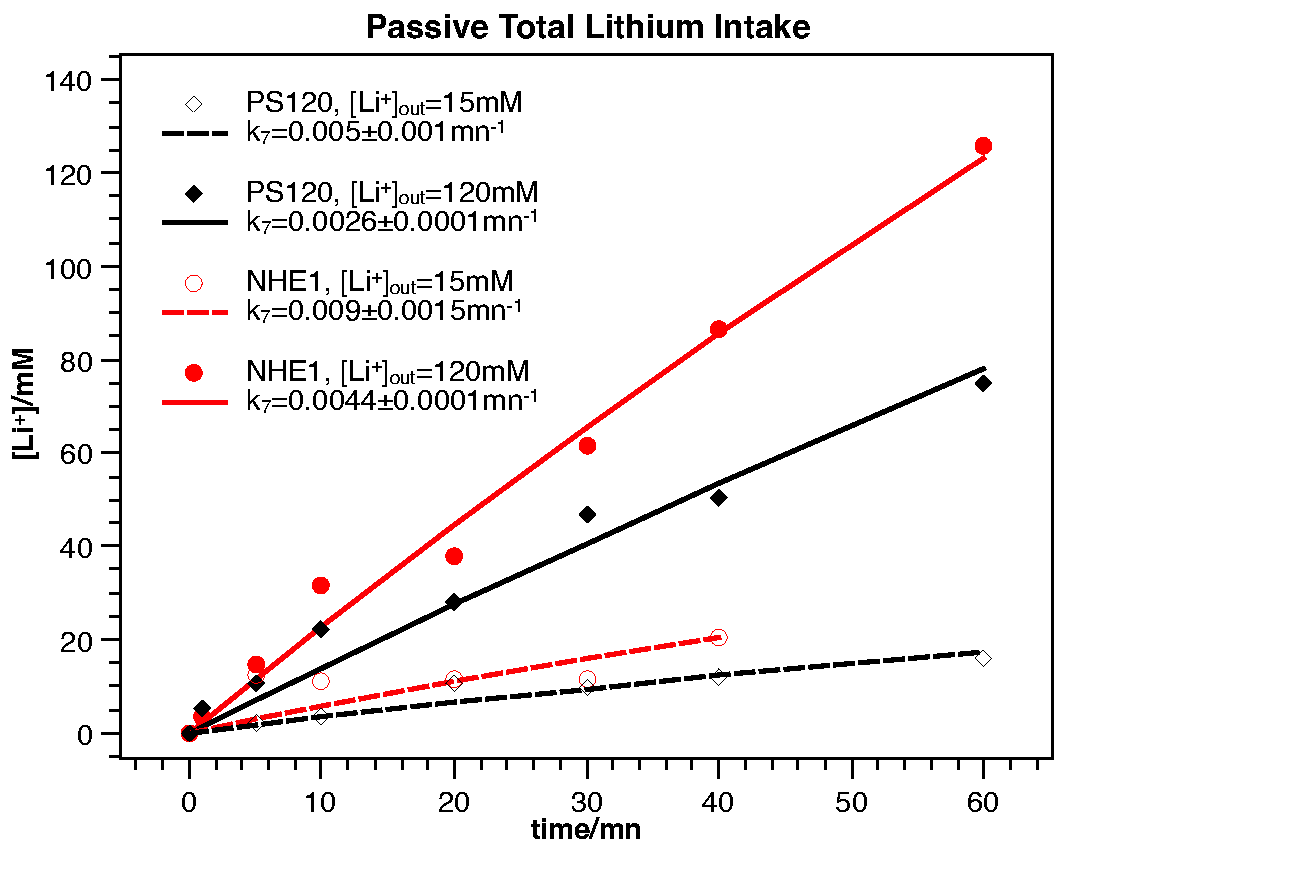
\includegraphics[width=0.5\textwidth]{leaks.pdf}
\end{center}
\caption{\label{fig:leak} Fit of experimental lithium electro-osmotic intake (points) according to the GHK theory (lines)}
\end{figure}
For different lithium concentrations and cell types, we find some consistent leak constants.
Moreover, a set of isotopic sepatations for $\mychem{PS120}$ cells at $\LiAllOut=120\text{mM}$ were measured after 1 minute and it amounts to:
\begin{equation}
\label{eq:d7ps120}
\deltaLi^\ko_{@1\text{mn}} = 12.6435 \pm 0.025.
\end{equation}
If we assume that
for this case $k_7\approx0.0026\,\text{mn}^{-1}$, then
\begin{equation}
	\sigma^\ko \approx 1.0019 \pm 2\cdot10^{-5},
\end{equation}
which is a very good approximation to the diffusive $\sigma=1.00229$. Accordingly, we will keep the more precise and documented $\sigma$ 
in the following theoretical and numerical work.

\section{Short Times Behaviours}

\subsection{Isotopic Separation}
We perform the short times integration of the system \eqref{eq:sysbis} using the initial
conditions \eqref{eq:ini} to get:
\begin{equation}
\beta_x(t) \underset{t\to0}{\approx} \left(k_x \Theta + E_0 \proton_0 \Upsilon_x\right) t,
\end{equation}
leading the initial ratio:
\begin{equation}
\label{eq:r0}
\left\lbrace
\begin{array}{rcl}
r_0 & = & \dfrac{k_7\Theta+E_0 \proton_0 \Upsilon_7}{k_6\Theta+E_0 \proton_0 \Upsilon_6}\\
	\\
    & = & \dfrac{k_7\Theta+E_0 \proton_0 \Upsilon_7}{ \sigma k_7\Theta+ \kappa E_0 \proton_0 \Upsilon_7}\\
\end{array}
\right.
\end{equation}







\end{document}
